% Springer Nature manuscript source, generated from the editable sections in this folder.
% Template version 3.1 (December 2024); no margin, font or spacing overrides.
\documentclass[pdflatex,sn-mathphys-num,iicol]{sn-jnl}
\usepackage{graphicx}
\usepackage{booktabs,tabularx,array}
\usepackage{amsmath,amssymb}
\usepackage{microtype}
\usepackage[title]{appendix}
\graphicspath{{figures/}}
% Allow compact, single-column floats to occupy available page space.
\setcounter{topnumber}{3}
\setcounter{bottomnumber}{2}
\setcounter{totalnumber}{5}
\setcounter{dbltopnumber}{3}
\renewcommand{\floatpagefraction}{.62}
\renewcommand{\dblfloatpagefraction}{.65}
\newcolumntype{Y}{>{\raggedright\arraybackslash}X}
\newcommand{\tabhead}[1]{\textbf{#1}}
\newcommand{\gaincell}[1]{\textbf{#1}}
\hypersetup{pdftitle={A Multi-Agent LLM Framework for SOC Threat Correlation and Alert Prioritization},pdfauthor={Hunain Shahid and Hammad Ullah Khan}}
\begin{document}
\title[A Multi-Agent LLM Framework for SOC Threat Correlation]{A Multi-Agent LLM Framework for SOC Threat Correlation and Alert Prioritization}
\author*[1]{\fnm{Hunain} \sur{Shahid}}\email{i240127@nu.edu.pk}
\author[1]{\fnm{Hammad Ullah} \sur{Khan}}\email{i242539@nu.edu.pk}
\affil*[1]{\orgdiv{Department of Artificial Intelligence and Data Science}, \orgname{National University of Computer and Emerging Sciences (FAST-NUCES)}, \orgaddress{\city{Islamabad}, \country{Pakistan}}}
\abstract{A SOC analyst has to decide which alerts describe the same incident before deciding what to inspect first. That decision can be distorted by copied observations, late-arriving evidence, and claims that disagree about an endpoint. We specify bounded correlation (C), prioritization (P), and verification (V) agent roles and test their software contracts with an offline adapter and a small local Qwen prototype. The measured experiment is separate: a frozen, deterministic C/V/P pipeline with a provenance gate. On a fresh synthetic holdout of 15 queues and 5,018 eligible alerts, its endpoint fallback raised incident Recall@20 from 250/300 (83.33\%) to \textbf{260/300 (86.67\%)}, recoverability from 263/300 (87.67\%) to \textbf{281/300 (93.67\%)}, and P@10 from 107/150 (71.33\%) to \textbf{113/150 (75.33\%)}. Neither arm formed a false grouped pair under simulator truth. After prediction files were sealed, an audit found 711 accepted genuine relationship tokens, no accepted false tokens, 35 genuine rejections, and 150 false rejections. The candidate had missed its development gate by one incident; testing it unchanged on the fresh holdout followed a documented protocol adjustment. A separate retrospective GUIDE reference reached 49.82\% Recall@20 on 499 queues. The local LLM run does not establish a model advantage, and the available GUIDE export lacks the original roots and evidence-arrival times required to test the frozen verifier on operational data.}
\keywords{security operations center, alert correlation, large language models, evidence provenance, multi-agent systems, incident prioritization}
\maketitle

\section{Introduction}
An analyst opening a SOC queue sees detector alerts, not neatly bounded incidents. Several alerts may describe one attack, but deciding which ones belong together is harder than finding a shared host or account. A second log entry, for example, may be a copy of the first; its event time may be early even though the entry reached the SOC after the decision was made. Treating either as independent, timely confirmation can merge two unrelated investigations. Existing work has studied aggregation, attack reconstruction, and triage from several angles \cite{landauer2022,wang2024,grain2025,sadlek2025}. Our starting point is the evidence behind an individual merge.

We therefore ask what can be joined using only evidence available at a fixed decision time. Correlation builds initial fragments and proposes further links. Verification checks whether each cross-fragment proposal has the required original observations and consistent fields. Only then does prioritization order the resulting groups for review. A better rank cannot recover an incident whose alerts were never grouped. This distinction matters because alert reduction, path reconstruction, severity prediction, and queue retrieval use different targets \cite{malach2025,grain2025,chuah2025}. Figure~\ref{fig:arch} shows the actual execution order.
\begin{figure*}[!tbp]\centering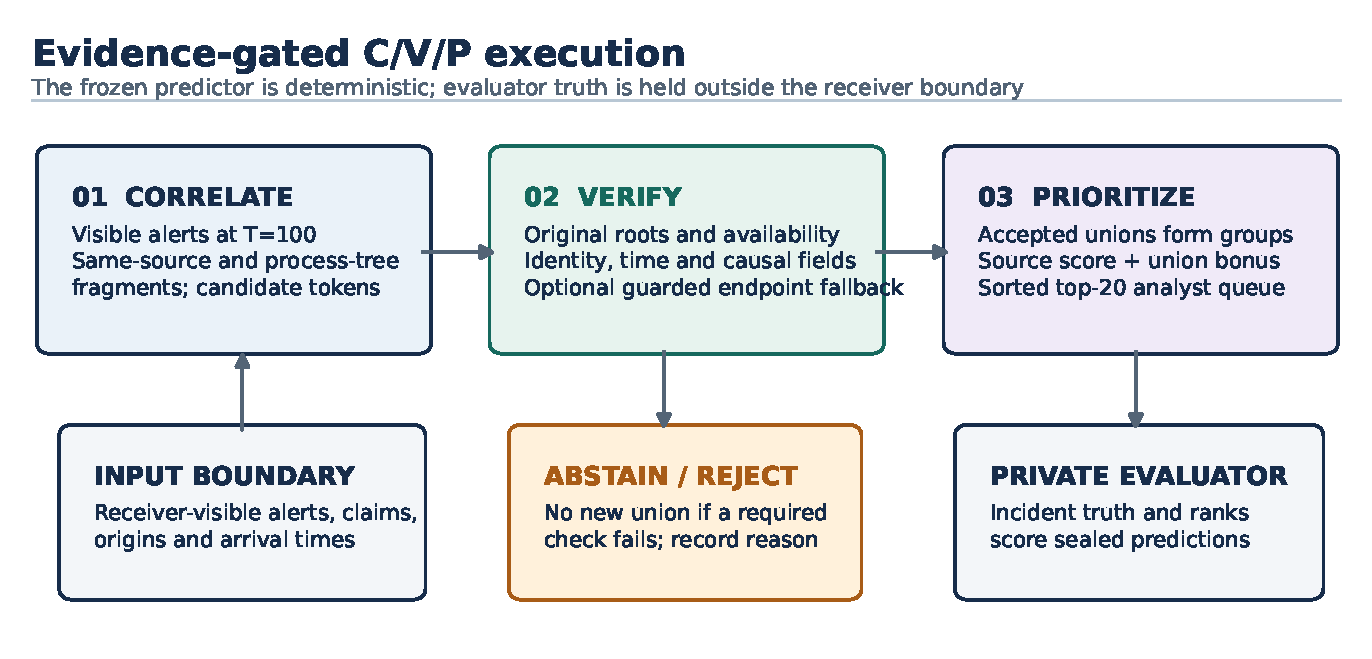
\includegraphics[width=.86\textwidth]{figures/architecture.pdf}\caption{Implemented C/V/P architecture. Receiver-visible alerts and claims enter initial correlation (C); independent-root, identity and temporal verification (V) controls additional fragment unions; prioritization (P) ranks the final groups. Rejected or insufficient bundles do not add a union. Private evaluator labels never enter prediction.}\label{fig:arch}\end{figure*}

Three questions guide the study. First, what does the verifier accept or refuse when claims are copied, late, missing, or inconsistent? Second, on the same untouched synthetic queues, does a narrowly defined endpoint fallback recover more incidents without an observed increase in incorrect groupings? Third, which missing data prevent the same test on a real SOC export? We contribute:
\begin{itemize}
\item bounded contracts for the three agent roles, alongside the rules actually executed by the frozen deterministic verifier;
\item a paired fresh holdout, reported at the incident, queue, group, and relationship-token levels, including queues where retrieval worsened;
\item an account of what the local LLM and GUIDE investigations did establish, and of the fields still needed for an external test.
\end{itemize}
The measured holdout does not compare our system with a published system on shared data. We keep that boundary explicit throughout the paper.


\section{Related work}
\subsection{Aggregation, reconstruction, and prioritization}
Landauer et al. learn aggregation patterns from semi-structured alerts \cite{landauer2022}; Wang et al. use similarity-based aggregation before Transformer-based attack prediction \cite{wang2024}; and GRAIN reconstructs multi-stage scenarios from a learned causal graph \cite{grain2025}. These studies motivate useful ways to organize a queue. Our experiment asks a narrower question about the evidence for a proposed edge: were the supporting observations original, independently rooted, and visible when the decision was taken? The studies use different inputs and evaluation targets, so their published scores are not direct comparators.

Other work starts from the triage decision itself: Sadlek et al. use kill-chain graphs to order incidents by severity \cite{sadlek2025}, while CyberShapley identifies informative parts of an anomaly graph \cite{malach2025}. In our evaluation, an incident must first have a sufficiently complete and pure group, and that group must then reach the first 20 queue positions. Provenance is also well established. HOLMES, POIROT, UNICORN, and CrossHound use information flows, audit trails, or host/network relationships for investigation \cite{holmes2019,poirot2019,unicorn2020,crosshound2026}. We build on that line of work by specifying a three-root decision gate with evidence-arrival time for this controlled grouping task; we do not claim to introduce provenance reasoning.

\subsection{Evidence assumptions and evaluation}
Reviews of security-event and log correlation document differences in data sources, missingness, and metrics \cite{review2022,chuah2025}. These differences are material here. A source ID does not prove that two real sensors are independent; the controlled generator supplies root identities, and the verifier rejects copies that trace back to the same root. The cited studies address aggregation, prediction, reconstruction, triage, or investigation with distinct labels and inputs; their published scores are not a same-data comparison with this experiment.


\section{Proposed methodology}
For queue $q$, let $A_q(T)$ be alerts whose ledger-recorded evidence availability minute is at most cutoff $T=100$. Each alert has an identifier, source identifier, observation identifier, event minute, host, account, process context, severity, and asset criticality. A relationship token $r=(a,b)$ is accompanied by claims from process, authentication, and network-flow families. A claim has an observation identifier, upstream-root identifier, optional \texttt{derived\_from} pointer, event-field assertions, and availability minute. Original means the derivation pointer is null; a derived copy remains dependent on its origin.

The algorithm outputs a partition $\mathcal G_q=(G_1,\ldots,G_m)$ of $A_q(T)$, ordered by a deterministic group score. Initial grouping uses source, process-tree, and selected lineage context; the extra verification stage is applied to cross-fragment claim tokens. An edge proposal is evidence for a possible union, whereas a group is a transitive partition component. The simulator's expert priority list and incident assignments are restricted to the evaluator. They are never model-visible fields.



Event time represents when the activity occurred; availability time represents when its supporting observation reached the receiver. A claim available at minute 105 is excluded at the minute-100 decision even if its event refers to minute 60.



\subsection{Agent framework and executable contracts}\label{sec:agents}
\subsubsection{Roles and evidence boundary}
A request contains opaque alert IDs, one approved evidence snapshot $E_T$, and explicit candidate, token, schema, prompt, and model-version budgets. The receiver rejects evaluator labels or lineage, cross-organization records, invalid citation IDs, duplicate keys, non-finite scores, excessive evidence, and unexpected JSON fields. Observation text is treated as data rather than an instruction. All roles receive the same cutoff-time snapshot.

For a supplied pair $(a,b)$, correlation (C) returns LINK, NO\_LINK, or UNSURE, with uncertainty, reason, and supporting/conflicting evidence IDs. It cannot search for new pairs. A bounded builder joins validated LINK edges; prioritization (P) scores the resulting candidate against other groups and cites its rationale. Verification (V) marks substantive claims supported, unsupported, unverifiable, or contradicted and returns PASS, REVISE, or REVIEW. At most one revision is allowed. Unresolved conflict, unsupported priority, invalid output, and provider failure route to review. The score is a ranking signal, not a calibrated attack probability.

For a request $x$, the contract requires $\mathcal A(x,E_T)=1$ only when every claim cites receiver-visible evidence that substantively supports it:
\begin{equation}\label{eq:citationgate}
\begin{aligned}
\mathcal A(x,E_T)=\mathbf1\bigl[\forall c\in\operatorname{claims}(x):{}&\\
\operatorname{cite}(c)\subseteq E_T\ \land\ {}&\operatorname{support}(c,E_T)\bigr].
\end{aligned}
\end{equation}
A cited ID alone is insufficient. PASS verifies this contract, not incident ground truth. Shared compromised sources and deceptive evidence text remain possible.

\subsubsection{Execution and measured scope}
The orchestrator validates pairs in stable order, records decisions and abstentions, permits one revision, and keys replay to input, role, schema, prompt, and model versions. Offline-adapter tests exercised four synthetic pairs, ten role calls, one revision, and one review; 34 assertions checked roles, citations, leakage, malformed output, caps, and replay, while 59 more checked evaluation and ranking boundaries. A bounded local \texttt{qwen2.5:3b} Ollama prototype ran on 20 organizations, but its pair universe differed from the statistical reference. Rules and BM25 have synthetic interfaces; single-call and repeated-call LLM controls use offline stubs. None of these contract tests establishes an LLM performance gain. The measured holdout instead uses the deterministic C/V/P path in Fig.~\ref{fig:arch}.


\subsection{Architecture and data flow}
Fig.~\ref{fig:arch} shows the computational order. The correlation routine first groups same-source alerts, process-tree references, and eligible lineage references with host/account guards and a component-size cap of 100. It returns a partition and candidate diagnostics. Verification then inspects each visible relationship-token bundle before any additional cross-fragment union. Finally the ranking routine orders the resulting groups for the analyst. The repository's earlier code labels this as C--P--V in places, but the frozen prediction call executes correlation, then verification, then scoring; we describe this actual execution order as C/V/P.

Verification outcomes in the implementation are reason-coded. A mismatched event or causal field, late claim, shared root, derived-only family, excessive component size, or incompatible component host/account context prevents union. An absent process claim may be considered by the constrained fallback in Section~\ref{sec:method}; its extra check uses receiver-visible endpoint fields, not truth labels. Rejected and insufficient proposals leave the existing partition intact. This is a conservative decision procedure under its assumed root semantics, not a formal guarantee against adversarially coordinated false observations.



\subsection{Evidence verification and endpoint fallback}\label{sec:method}
\subsubsection{Visibility and initial fragments}
Before correlation, the receiver checks that the evidence ledger is contiguous, has one availability entry per alert, agrees with alert-level availability, and contains no private fields. At cutoff $T=100$, it keeps only arrived alerts and claims whose two endpoints are eligible. The initial pass groups same-source and process-tree fragments, then considers available lineage references. Host, account, and size guards apply to the components at that stage. The later claim verifier does not go back and certify every pair made within a source. This matters when interpreting the zero false-pair result: it was observed in the holdout, not guaranteed by the verifier's logic.

\subsubsection{Original independent attestation}
For each proposed relationship, the baseline inspects a bundle of claims. To join two fragments it needs one original process claim, one original authentication claim, and one original network claim, all from different upstream roots and all available by $T$. Endpoint and event identities, host, account, process parent, session, and flow fields must agree. The event-time check is $t_b\geq t_a-3$ and $|t_b-t_a|\leq25$ minutes. A copy of an original observation does not supply a missing family. Finally, the two current components must overlap on host and account and contain at most 100 alerts after union.

The root and visibility checks are necessary conditions:
\begin{equation}\label{eq:gate}
\begin{aligned}
\left|\{\rho(c):c\in B_r,\;c\text{ original}\}\right|&=3,\\
\max_{c\in B_r}t_{\mathrm{available}}(c)&\leq T.
\end{aligned}
\end{equation}
The two conditions in (\ref{eq:gate}) are only part of the decision. Identity, context, event time, and component guards must also pass. On failure the verifier records a reason and makes no union. It checks each token against original alert fields; a newly enlarged group cannot serve as a new witness for the next token. Group membership is nevertheless transitive after independently checked unions, so one final group may contain several fragments.

\subsubsection{Constrained endpoint fallback}
The candidate revisits just one failure reason: \texttt{missing\_family}. If the process claim is absent, it may use original endpoint observations alongside one original authentication and one original network-flow claim. The two claims must have different roots and be available by minute 100. The endpoints must be original, have different source and observation IDs, and share an endpoint-origin root distinct from both claim roots. Host, account, event timing, process parent, session, and flow must agree between endpoints and claims. The existing component guards still apply. Thus the endpoint context fills the missing process-family role; it cannot excuse a contradiction, a late claim, or another failure. Figure~\ref{fig:verify} shows the branches.
\begin{figure*}[!tbp]\centering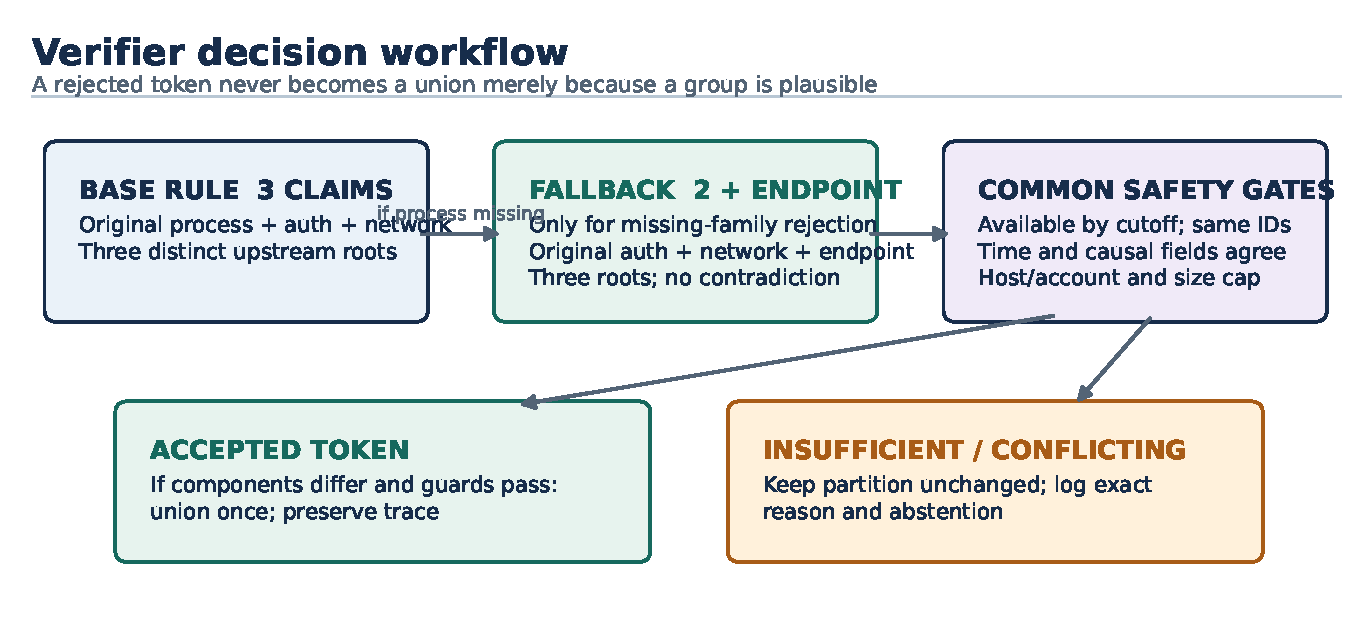
\includegraphics[width=.88\textwidth]{figures/verification_methodology.pdf}\caption{Frozen verifier workflow. The baseline requires original process, authentication and network claims from three distinct roots. Only \texttt{missing\_family} can trigger the fallback: original authentication and network claims plus a distinct original endpoint root. Identity, event-time, availability, causal fields, component context and size gates still apply. Failure leaves the partition intact. Evaluator truth is unavailable to prediction.}\label{fig:verify}\end{figure*}

\subsubsection{Decision semantics and component state}
Claim validity and permission to merge are separate checks. A valid token may point to alerts already in one component; then there is nothing to join. It may also pass its claim checks but fail because the proposed combined group would exceed 100 alerts or the components have no host/account overlap. Existing groups stay intact in either case. Bundles are processed in sorted order, with union--find tracking the additional verified joins. The three-root requirement counts the original observations for a token, not alerts accumulated in its component.

An authentication copy retains its upstream root; a late claim is unavailable even when its event time is early. Contradictory causal fields block a union. Only an absent process-family witness can trigger the guarded endpoint substitution.


\subsubsection{Grouping and scoring}
Both arms retain one representative per source, apply the same fixed score, and sort by descending score then first alert ID. Each accepted token whose left endpoint belongs to the group adds one point. Fallback can alter the partition and token count; ranking alone cannot make an unrecoverable incident recoverable.
For group $G$, let $D(G)$ denote the code's one-alert-per-source representatives, $s(a)$ and $c(a)$ the alert severity and criticality, $E(D)$ the distinct event types in those representatives, and $U(G)$ the accepted tokens whose left endpoint belongs to $G$. The implemented score in both primary arms is
\begin{equation}\label{eq:score}
\begin{aligned}
F(G)={}&1.2\max_{a\in D(G)}s(a)+0.7\max_{a\in D(G)}c(a)\\
&+0.55|E(D(G))|+0.7\min\{|D(G)|,10\}\\
&+|U(G)|.
\end{aligned}
\end{equation}
The fallback can change both $G$ and $U(G)$, so a changed rank is not isolated evidence of a superior ranking function. The fixed ranking expression is a deterministic heuristic, not a learned probability of incident severity.



\section{Experimental setup}
We generated queues with process, authentication, and network-flow claims. The generator also recorded whether an observation was original or derived, when it became available, and whether fields were missing or contradictory. Eight training queues and ten development queues informed the method. On the latter, the candidate recalled 169 of 200 expert top-20 incidents, recovered 177, and credited 73 of 100 P@10 positions; it had no false grouped pairs or mixed groups. The planned gate was 170/200 Recall@20, so the candidate missed it by one incident. The team documented a decision to test the candidate unchanged on a new holdout. We report this as a protocol adjustment, not a gate pass.

The fresh sample used seed 31103 and template variant 2: \textbf{15 queues}, \textbf{5,018 cutoff-eligible alerts}, and 300 expert top-20 incident opportunities. Both methods received identical inputs. Source/configuration hashes were fixed and prediction files SHA-256 sealed before private truth was opened. Each arm ran once; the holdout remains within the generator family. Its audit recorded 345 false independent-looking claims, 170 derived copies, 95 false same-context tokens, 55 late claims, and 28 missing true claims. These overlapping challenge categories are not a partition.



\subsection{Dataset, parameters, and reproducibility}\label{sec:reproduce}
The controlled evidence generator is the dataset source for the primary experiment. Its configuration fixes 25 incidents and 60 benign events per queue, the minute-100 decision cutoff, and a maximum component size of 100. The training split uses eight queues (seed 31101, template variant 0), development ten (seed 31102, variant 1), and the frozen test 15 (seed 31103, variant 2). The test generator emitted 5,039 alerts and 2,752 claim records; 21 alerts arrived after the cutoff, leaving 5,018 eligible. The generator audit also records 55 late claims, 170 derived claim copies, 28 missing true claim records, 345 false independent-looking claim records, and 95 same-context false tokens. These are properties of the synthetic sample, not real SOC frequencies.

The predictor uses the thresholds in Sections~\ref{sec:method} and the fixed coefficients in (\ref{eq:score}); it does not fit a model on the test split. Both methods start from the same 2,685 candidate pairs. The comparator is the frozen \texttt{evidence\_aware\_ranked} pipeline; the candidate adds the \texttt{missing\_family} endpoint rule and retains the verified-token score bonus of 1. Prediction runs with Python 3.12 standard-library code. The repository pins Matplotlib 3.11.2 and NumPy 2.5.4 for figures; neither library is needed by the frozen predictor. We do not infer portable latency from the single recorded executions, whose hardware specification was not archived.

The source repository is \url{https://github.com/Hunain230/CN-Research-}. Within it, \path{experiments/PHASE33_FROZEN_GENERALIZATION/} contains \texttt{config.json}, \texttt{PHASE33\_FREEZE.json}, the generator, \texttt{run\_holdout.py}, the original queue CSV, prediction and evaluation artifacts, and the pre-evaluation SHA-256 seal. The models reside in the Phase 31 and 32 experiment directories; the unchanged evaluator is in \path{experiments/PHASE15_CONTROLLED_SOC/evaluation/evaluate.py}. The one-shot runner refuses to overwrite existing predictions. We also ran a same-seed replay in an isolated temporary directory: its manifest and all 15 per-queue recall, recoverability, and P@10 counts matched the archive, as did the aggregate grouping-safety counts. This is a reproducibility check of the original cohort, not a second independent holdout. The replay and paired bootstrap scripts are included under \texttt{analysis/} in this package.


\subsection{Evaluation metrics}
The evaluator has 25 expert-priority incidents per queue and takes ranks 1--20 as the target set. Let $n_i$ be the number of eligible alerts for incident $i$, $h_{iG}$ the number of those in predicted group $G$, and $|G|$ its size. A group qualifies for $i$ if
\begin{equation}\label{eq:qualify}Q(i,G)=\mathbf{1}\left[\frac{h_{iG}}{n_i}\geq0.8\;\land\;\frac{h_{iG}}{|G|}\geq0.8\right].\end{equation}
The denominator $n_i$ concerns eligible alerts, not all generated alerts. Every expert incident must have at least one eligible alert. If any group qualifies, $i$ is recoverable; if any qualifying group has rank at most 20, it is recalled. For $N$ queues, let $\mathcal G_q^{20}$ be the groups ranked at most 20 and $I_q^{20}$ the 20 expert-priority incidents. The implementation micro-aggregates counts:
\begin{align}\label{eq:recall}
R@20&=\frac{1}{20N}\sum_q\sum_{i\in I_q^{20}}
\max_{G\in\mathcal G_q^{20}} Q(i,G),\\
\operatorname{Recov}&=\frac{1}{20N}\sum_q\sum_{i\in I_q^{20}}
\max_{G\in\mathcal G_q} Q(i,G).
\end{align}
For P@10 the evaluator scans the first 20 groups, credits at most one previously uncredited qualifying incident per group (lowest expert rank if several qualify), and counts a credit only when the group is within positions 1--10 and the incident's expert rank is at most 10. The aggregate denominator is $10N$. This assignment rule is more specific than ordinary binary relevance precision.

For each group, the evaluator counts true within-group pairs $\sum_i\binom{h_{iG}}2$ and false within-group pairs $\binom{|G|}2-\sum_i\binom{h_{iG}}2$. Grouped-pair precision is total true divided by total true plus false pairs across queues; its implementation defines precision as one when no pairs exist. False grouped pairs is the summed false count. A mixed group is any predicted group containing more than one truth incident, even if it passes the 80\% purity threshold. These safety measures include all groups, not just the top 20. Candidate-edge precision is not recoverable from the prediction artifact and is not reported.


\section{Results and analysis}
\subsection{Primary frozen synthetic holdout}
Table~\ref{tab:primary} compares matched predictions. The fallback recovers 18 more expert incidents somewhere in the output, retrieves ten more by rank 20, and credits six more in the first ten positions: \textbf{+6.00 points recoverability}, \textbf{+3.33 points Recall@20}, and \textbf{+4.00 points P@10}. These measures use distinct denominators.

Figure~\ref{fig:bootstrap} reports a descriptive paired-queue bootstrap. For metric $M$, the effect is $\hat\Delta_M=15^{-1}\sum_{q=1}^{15}(M_{q,\mathrm{fallback}}-M_{q,\mathrm{base}})$ in percentage points; 10,000 queue resamples with replacement (seed 31103) yield percentile intervals. The 95\% intervals are \textbf{[0.67, 6.00]} for Recall@20, \textbf{[4.00, 8.00]} for recoverability, and [-0.67, 8.67] for P@10. The last crosses zero. These conditional intervals do not establish a real-SOC error bound or a second independent holdout.
\begin{table*}[!tbp]\centering\footnotesize\caption{Frozen paired holdout results. Fractions use evaluator opportunity denominators. Differences are candidate minus baseline; percentage differences are percentage points.}\label{tab:primary}\begin{tabularx}{\textwidth}{@{}Yrrr@{}}\toprule Metric & Frozen baseline & Endpoint fallback & Difference\\\midrule Incident Recall@20 & 250/300 (83.33\%) & \gaincell{260/300 (86.67\%)} & \gaincell{+10 (+3.33 pp)}\\ Group recoverability & 263/300 (87.67\%) & \gaincell{281/300 (93.67\%)} & \gaincell{+18 (+6.00 pp)}\\ P@10 & 107/150 (71.33\%) & \gaincell{113/150 (75.33\%)} & \gaincell{+6 (+4.00 pp)}\\ Grouped-pair precision & 19,459/19,459 (100\%) & 20,117/20,117 (100\%) & 0 pp\\ False grouped pairs & 0 & \gaincell{0} & 0\\ Mixed groups & 0 & \gaincell{0} & 0\\\bottomrule\end{tabularx}\end{table*}

\begin{figure}[!htbp]\centering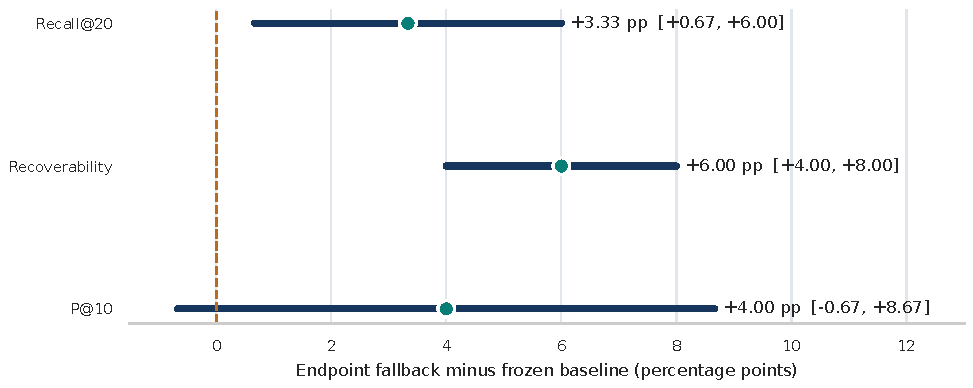
\includegraphics[width=.98\columnwidth]{figures/paired_bootstrap_intervals.pdf}\caption{\textbf{Paired-queue effects and uncertainty.} Point estimates are candidate minus baseline; lines are descriptive percentile intervals from 10,000 queue resamples. Recall/recoverability use 300 incident opportunities and P@10 uses 150 rank positions. The dashed line denotes zero effect.}\label{fig:bootstrap}\end{figure}
Figure~\ref{fig:rankpanels} shows the full rank-cutoff behavior. Both arms retrieved 75/300 expert incidents by rank five; the counts were 143 versus 148 by rank ten and 250 versus 260 by rank 20. The interval bars show where newly qualifying incidents entered the reviewed queue.
\begin{figure*}[!tbp]\centering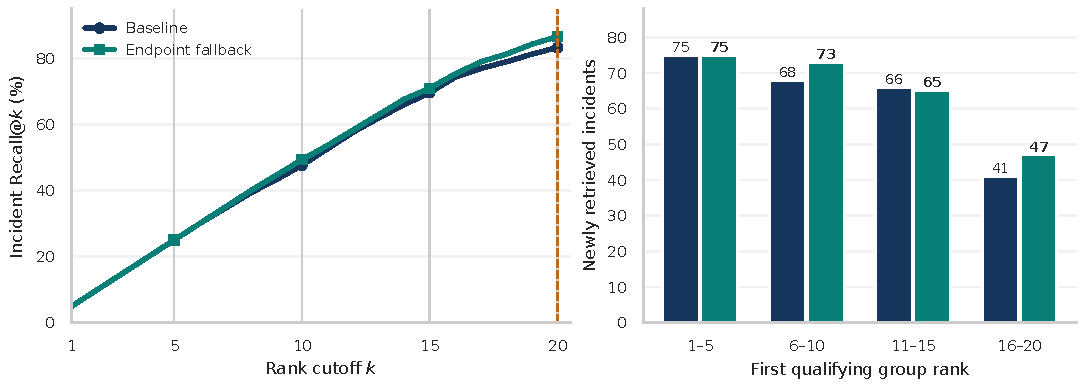
\includegraphics[width=.83\textwidth]{figures/rank_retrieval_panels.pdf}\caption{\textbf{Ranked incident retrieval on the paired holdout.} Left: cumulative expert-incident Recall@$k$ from the sealed ranked groups. Right: newly retrieved incidents by first qualifying group position. Each arm has the same 300 expert top-20 opportunities; bars partition its own Recall@20 count.}\label{fig:rankpanels}\end{figure*}
After predictions were sealed, the truth audit found that \textbf{all 28 new fallback unions}, and all 711 accepted candidate tokens overall, were genuine under simulator labels. The verifier rejected 150 false tokens and also abstained on 35 genuine ones. Tokens are proposals; they should not be confused with the much larger set of pairs inside final groups. Both arms had \textbf{zero false grouped pairs and zero mixed groups} in all 15 queues. That clean grouping result did not prevent local ranking losses: two queues each lost one recalled incident, and P@10 decreased in two queues.


\subsection{Decision confusion matrix and paired outcomes}
Table~\ref{tab:confusion} gives the 896 token decisions in the sealed candidate run. Here ``positive'' means that the verifier accepted a proposed relationship, not that a detector labeled an alert malicious. Of the 711 accepted proposals, 28 are unions admitted by the fallback; none was false under simulator truth. Thirty-five genuine proposals were rejected or left unresolved because the evidence did not satisfy the rule, while 150 false proposals were rejected. Conditional acceptance precision is $711/(711+0)=100\%$, recall among genuine proposed tokens is $711/(711+35)=95.31\%$, and rejection specificity among false proposed tokens is $150/(150+0)=100\%$. These denominators cover submitted tokens only, not every alert pair or an operational population.
\begin{table}[!htbp]
\centering\footnotesize\caption{Candidate token-decision confusion matrix on the frozen synthetic holdout; truth opened only after predictions were sealed. Rows are verifier decisions; columns are simulator truth.}\label{tab:confusion}
\begin{tabular}{@{}lrr@{}}\toprule
 & Genuine & False\\\midrule
Accepted & \gaincell{711 (TP)} & 0 (FP)\\
Rejected/abstained & 35 (FN) & \gaincell{150 (TN)}\\\bottomrule
\end{tabular}
\end{table}
Figure~\ref{fig:outcomepanels} separates group recoverability from rank placement and shows the paired incident transitions. Both arms retrieved 245 incidents; the candidate alone retrieved \textbf{15}, the baseline alone five, and neither retrieved 35. There are no designated negative incident opportunities, so these counts do not yield classification accuracy or true negatives. We also do not infer pair recall without the eligible same-incident pair denominator.
\begin{figure}[!htbp]\centering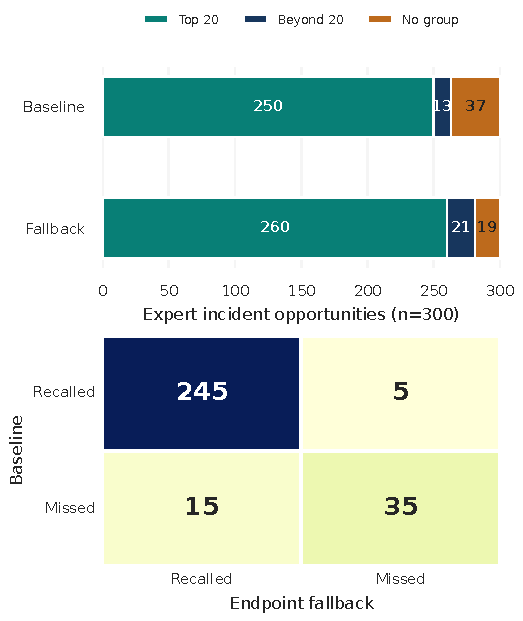
\includegraphics[width=.98\columnwidth]{figures/incident_outcome_column.pdf}\caption{\textbf{What changed for the same 300 expert incidents.} Top: each arm's disjoint top-20, below-20 but recoverable, and unrecoverable outcomes. Bottom: paired Recall@20 decisions, where off-diagonal cells expose gains and losses. The matrix is incident retrieval, not token-decision confusion.}\label{fig:outcomepanels}\end{figure}
The frozen summary additionally reports nDCG@20 of 0.8852 versus 0.9201 and MRR of 1.0 in both arms. It records 1,333 versus 1,305 predicted groups and 683 versus 711 accepted merges. Its recorded run durations of 0.696 and 0.656 seconds are single execution measurements, with no repeated-run uncertainty or hardware-normalized latency claim.
\subsection{Where the aggregate gains arose}
The heatmap in Figure~\ref{fig:queueheat} shows integer differences for each queue. Recall improved in eight queues, tied in five, and fell by one in two. Recoverability improved in twelve and tied in three. P@10 improved in five, tied in eight, and fell in two. Each queue contributes 20 possible incidents to Recall@20 and recoverability, but only ten possible credits to P@10. The plot makes visible the cases hidden by an aggregate gain.
\begin{figure*}[!tbp]\centering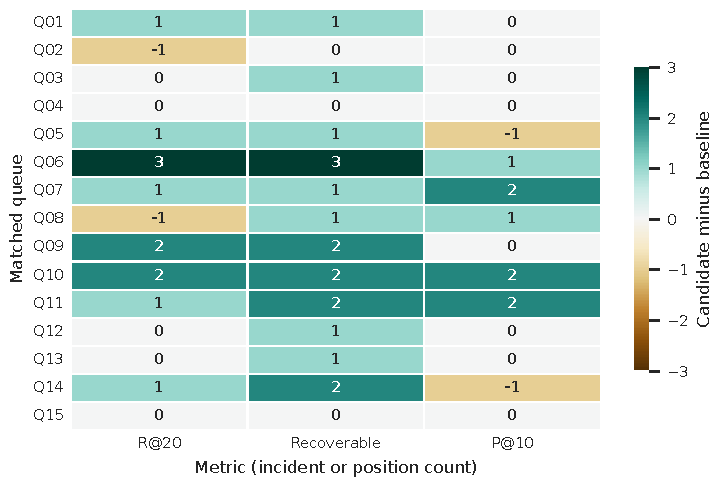
\includegraphics[width=.76\textwidth]{figures/queue_delta_heatmap.pdf}\caption{\textbf{Paired queue differences:} each cell is candidate minus baseline, from the archived queue CSV. Blue-green marks gains, brown losses and white no change; integers remain readable without color. Queue numbering is display order, not a time series.}\label{fig:queueheat}\end{figure*}
The baseline's 263 recoverable incidents split into 250 retrieved by rank 20 and 13 below it; the candidate's 281 split into 260 and 21. Thus the count lacking any qualifying group fell \textbf{37 to 19}, but recoverable incidents below the retrieval cutoff rose 13 to 21. Group reconstruction and score order both changed, so this does not isolate an individual ranking failure.

\subsection{Development-only and historical evidence}
Separate development studies examined ranking and evidence rules. Their scores are not substituted for the frozen holdout or construed as a performance trajectory. The earlier historical synthetic holdout had 407/600 Recall@20 and 451/600 recoverability on another population; its scores are not directly comparable. An unsafe richer-claim development configuration produced 2,580 false pairs and 22 mixed groups, whereas independent-claim verification on that development cohort preserved zero false pairs and recovered 166/200 incidents.



\section{Comparison with base papers and state of the art}\label{sec:base}
We chose Hmimou et al. \cite{hmimou2025} as the primary base paper in the Phase 1 review because it puts specialized LLM agents to work on threat correlation. Its email, log, and IP agents combine LLaMA 3.3-70B with retrieval and security tools. On the authors' evaluation, the reported figures are 93.6\% system accuracy, 87.0\% correlation precision, 41.3\% fewer false positives, and 38.5\% less analyst triage time than their SIEM control. Their question is broader than ours, but their study does not test whether a sufficiently complete expert-priority incident reaches the top 20 of a ranked queue. The four figures belong to their experiment and are not our results.

Guo et al. \cite{guo2026} helps frame the other half of our topic, alert priority. Their system combines an FFT--PCC risk gate, BERT-assisted evidence handling, graph context, and AHP ranking; they report F1 of 0.910 for false-positive identification and a separate 45.2\% response-time reduction. Its online components are function-specific rather than an autoregressive generative LLM pipeline. AgentSOC by Roy and Singh \cite{agentsoc2026} instead generates hypotheses and ranks response actions after structural simulation. Neither paper reports the expert-labeled top-20 incident-queue outcome used here.

Our extension makes the evidence gate explicit at receiver time and evaluates both grouping and queue retrieval. Against our own matched synthetic baseline, endpoint fallback adds 3.33 percentage points to R@20 (4.0\% relative), 6.00 points to recoverability, and 4.00 points to P@10. This is not a numerical improvement over Hmimou et al.: we did not run their implementation on the same observations, candidate universe, labels, or metrics. The small local prototype also cannot tell us whether three LLM roles outperform one. A shared-data comparison remains a separate experiment.


\section{Ablation study}\label{sec:ablation}
The ten development queues hold the cohort fixed while varying the evidence rule (Fig.~\ref{fig:ablation}). Rich claims connected more fragments but produced \textbf{2,580 false within-group pairs} and 22 mixed groups. Independent-root verification removed those observed errors and yielded 158/200 Recall@20 with a fixed rank bonus. Endpoint fallback then raised Recall@20 to \textbf{169/200} and recoverability from 166/200 to \textbf{177/200} on the same queues; its 14 new unions were genuine under generator truth. It missed the planned 170/200 development gate by one. No development count is added to the fresh holdout.
\begin{figure*}[!tbp]\centering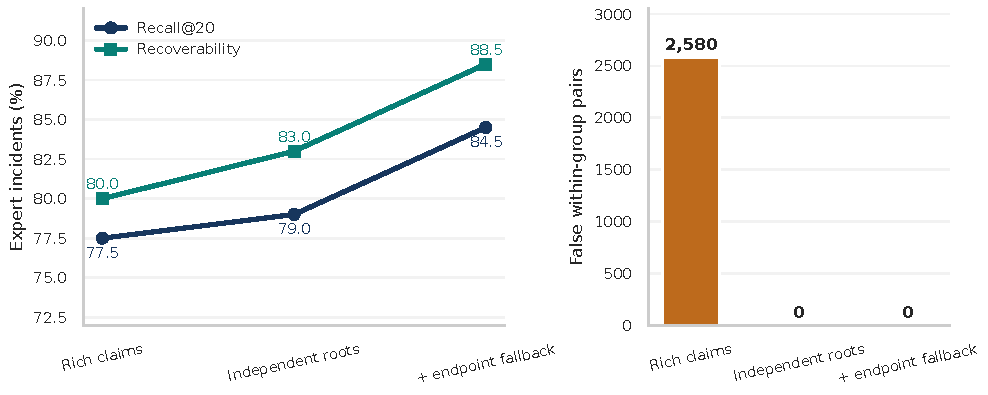
\includegraphics[width=.72\textwidth]{figures/development_ablation.pdf}\caption{\textbf{Matched development ablation on ten queues.} Left: incident Recall@20 and group recoverability (denominator 200). Right: false within-group pairs across all predicted groups. The rich-claim variant is unsafe; the last two variants have zero observed false pairs. These are development results, separate from the 15-queue holdout.}\label{fig:ablation}\end{figure*}
Other investigations used separate development cohorts. One hard-negative ranker left groups unchanged but moved matched R@20 from 263/300 to 262/300. Delaying or removing independent evidence also reduced reconstruction. We do not pool those trials with the primary holdout or describe them as holdout ablations. There is still no eligible real-queue comparison of C/P/V against a single LLM, so the contribution of LLM agent count has not been measured.


\section{Discussion}
The guarded endpoint substitution added 18 recoverable incidents but ten top-20 recalls. The eight-incident difference shows that reconstruction and ranking are separate bottlenecks. Zero observed false pairs does not establish independence of real upstream sources.

Copies retain their root and late evidence is invisible regardless of event time. Delayed, missing, or contradictory observations reduced recovery in development. A pairwise-trained ranker moved matched development Recall@20 from 263/300 to 262/300 with unchanged groups, illustrating objective mismatch.

The strict rule rejected or abstained on 35 genuine proposed tokens. Analyst preference for this tradeoff depends on telemetry and missed-incident cost, neither measured here.


\subsection{Threats to validity}
The generator supplies truth, roots, and causal fields. Three simulated roots may correspond to dependent or compromised real feeds; the fresh template variant remains within the development generator family. Fifteen queues cannot bound an operational error rate.

Testing despite a one-incident development-gate miss was a recorded protocol adjustment before holdout generation. Results depend on the 80\% completeness/purity rule and simulated priority labels. Large groups dominate pair counts, and initial within-source groups bypass the later three-root verifier. Distinct diagnostic cohorts are not paired with this holdout.

Real false unions, analyst benefit, workload, latency distribution, and abstention cost remain unmeasured.


\subsection{External evaluation readiness}
The local Microsoft GUIDE export contains 4,147,992 evidence rows, 637,320 composite alert keys, and 9,980 ranking rows. Of the alert keys, 70,702 have conflicting incident assignments. Timestamp perturbation \cite{guide2024} and the absence of evidence-arrival times, original roots, derivation chains, and causal claim bundles prevent an equivalent point-in-time verifier evaluation. Queue/rank semantics and approved model-visible fields also remain unresolved.



No GUIDE prediction or real-data performance result is attributed to the frozen verifier.


\section{Conclusion and future work}
In this controlled study, an endpoint observation could sometimes stand in for a missing process claim without relaxing the checks for timely, original, mutually consistent evidence. On the fresh synthetic queues, that rule raised \textbf{Recall@20 from 250/300 to 260/300} and \textbf{recoverability from 263/300 to 281/300}; neither arm produced a false grouped pair or mixed group under simulator truth. The candidate missed its development gate, and we have disclosed the decision that allowed its unchanged holdout test. These results establish a bounded synthetic finding, not a measured LLM or real-SOC advantage. The next useful test would collect authorized point-in-time evidence with documented upstream roots and predeclare the comparison before new queue labels are opened.


\section{Declarations and acknowledgements}
\paragraph{Data and code availability.} The public Microsoft GUIDE release is cited in the references. The controlled generator, configuration, per-queue results, prediction hashes, sealed summaries, and evaluator source are maintained at \url{https://github.com/Hunain230/CN-Research-}; Section~\ref{sec:reproduce} identifies the experiment paths. Authors should verify repository access and redistribution permissions at submission. The controlled holdout includes evaluator-only truth and should be shared under a protocol that preserves the intended test boundary.
\paragraph{Funding and competing interests.} Funding and competing-interest disclosures require author confirmation before submission; no declaration is inferred from the project files.
\paragraph{AI-assisted tools.} AI-assisted drafting and coding tools were used in the research and manuscript workflow. The authors must review the final wording, source attributions, figures, calculations and venue-specific disclosure policy before submission. The tools are not authors and no generated claim substitutes for an experimental artifact.
\paragraph{Acknowledgements.} The authors should add any human contributors and institutional support after confirmation. No unverified acknowledgement is inserted.

\bibliography{references}
\end{document}
